\begin{figure}[h]
    \centering
    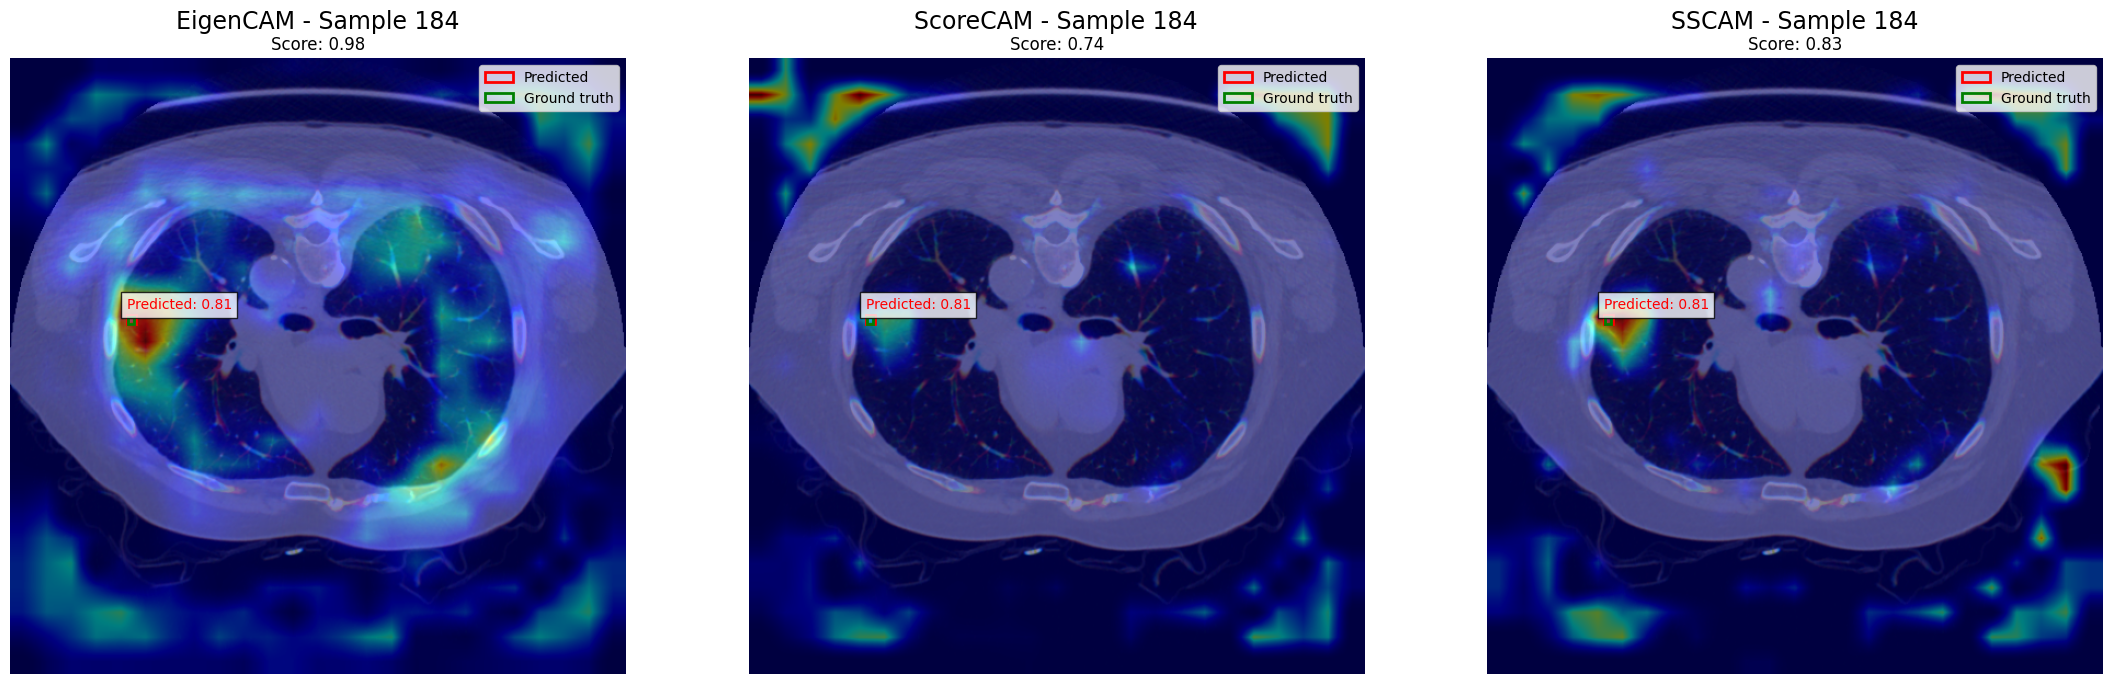
\includegraphics[width=1\linewidth]{images/xai-sample-184.png}
    \caption{Qualitative comparison of CAM methods on a representative test sample (Sample 184). The model's prediction is shown in red, and the ground truth in green. The Inverse Distance Score for each explanation is displayed at the top. \textbf{(Left)} Eigen-CAM, despite producing a heatmap that looks noisier than the others, has its focus right on the nodule (Score: 0.98). \textbf{(Center)} Score-CAM's heatmap has less noise, but its top activations are scattered away from the nodule (Score: 0.74). \textbf{(Right)} SS-CAM shows a minimal smoothing with respect to Score-CAM, but a higher concentration on the point of interest (Score: 0.83)}
    \label{fig:xai-qualitative-example}
\end{figure}